\section{Part 1: Brain Signal (EEG)}

\begin{taskbox}[Part 1: introduction in the lab manual]
A segment of EEG is provided in the file \texttt{sig\_EEG.mat}. The file contains a matrix \texttt{Z}, a 32-channel signal over time samples. The sampling frequency and the channel labels (in channel order) are stored in the variable \texttt{des}. The signal belongs to an epileptic patient and was recorded before and during a seizure. Since the signal is real, muscle artifacts are clearly visible in it.
\end{taskbox}

\subsection{Question 1: Displaying Channel 5}
\begin{taskbox}
Plot the signal of the 5th channel in the time domain. Set the time axis so that it is displayed in seconds. Set the figure height and width manually so that the changes of the signal shape over time are clearly visible. Write the channel label as the y-axis label or the figure title.
\end{taskbox}

According to the data labels, channel 5 is C3; this name refers to the left central region of the hemisphere in the electrode naming scheme. Figure~\ref{fig:c3full} shows the complete 64-second recording with the time axis in seconds. The differences in waveform shape across the recording, and the growth of amplitude in the later parts, can be seen. The last sample lies at 63.9961 seconds, and the recording length follows from the number of samples divided by the sampling rate.

\begin{figure}[H]
\centering
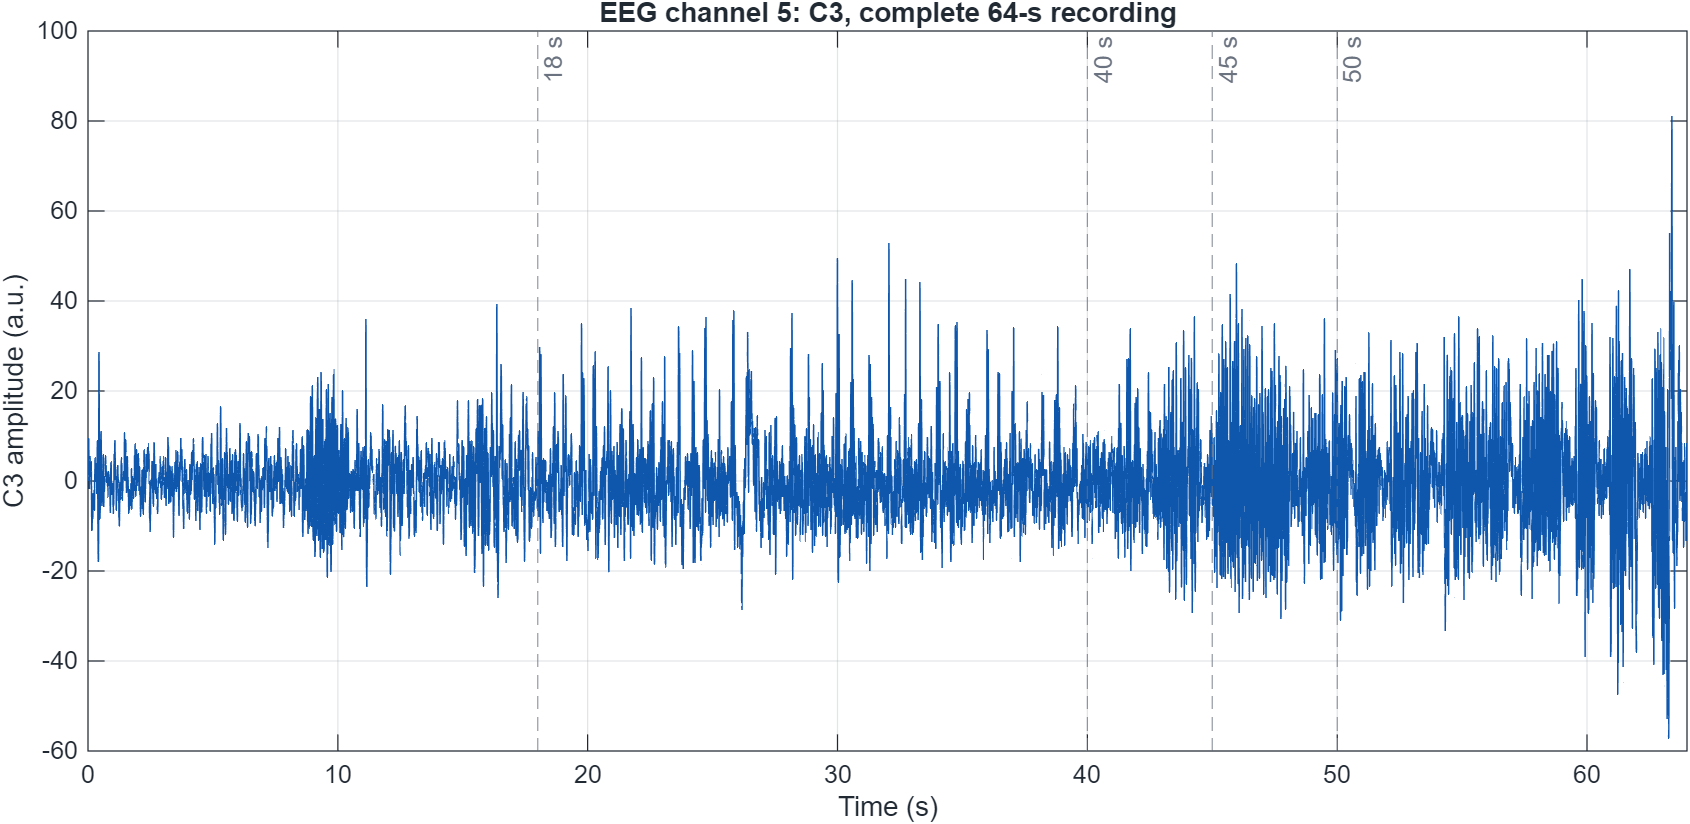
\includegraphics[width=\textwidth]{fig01_c3_full_recording.png}
\caption{Time display of the complete channel 5 (C3) and approximate boundaries for the morphology examination.}
\label{fig:c3full}
\end{figure}

\paragraph{Time--frequency spectrogram of the whole C3 signal.} To complete the time display, Figure~\ref{fig:c3stft} shows the distribution of power density over the entire 64-second recording. A two-second Hamming window with a 0.25~s step was used, and the mean of each window was removed. A warmer color indicates a greater power density; the color value is in dB relative to $1\ \mathrm{a.u.}^2/\mathrm{Hz}$ and is not the direct amplitude of the wave. For example, 10~dB corresponds to $10\ \mathrm{a.u.}^2/\mathrm{Hz}$.

\begin{figure}[H]
\centering
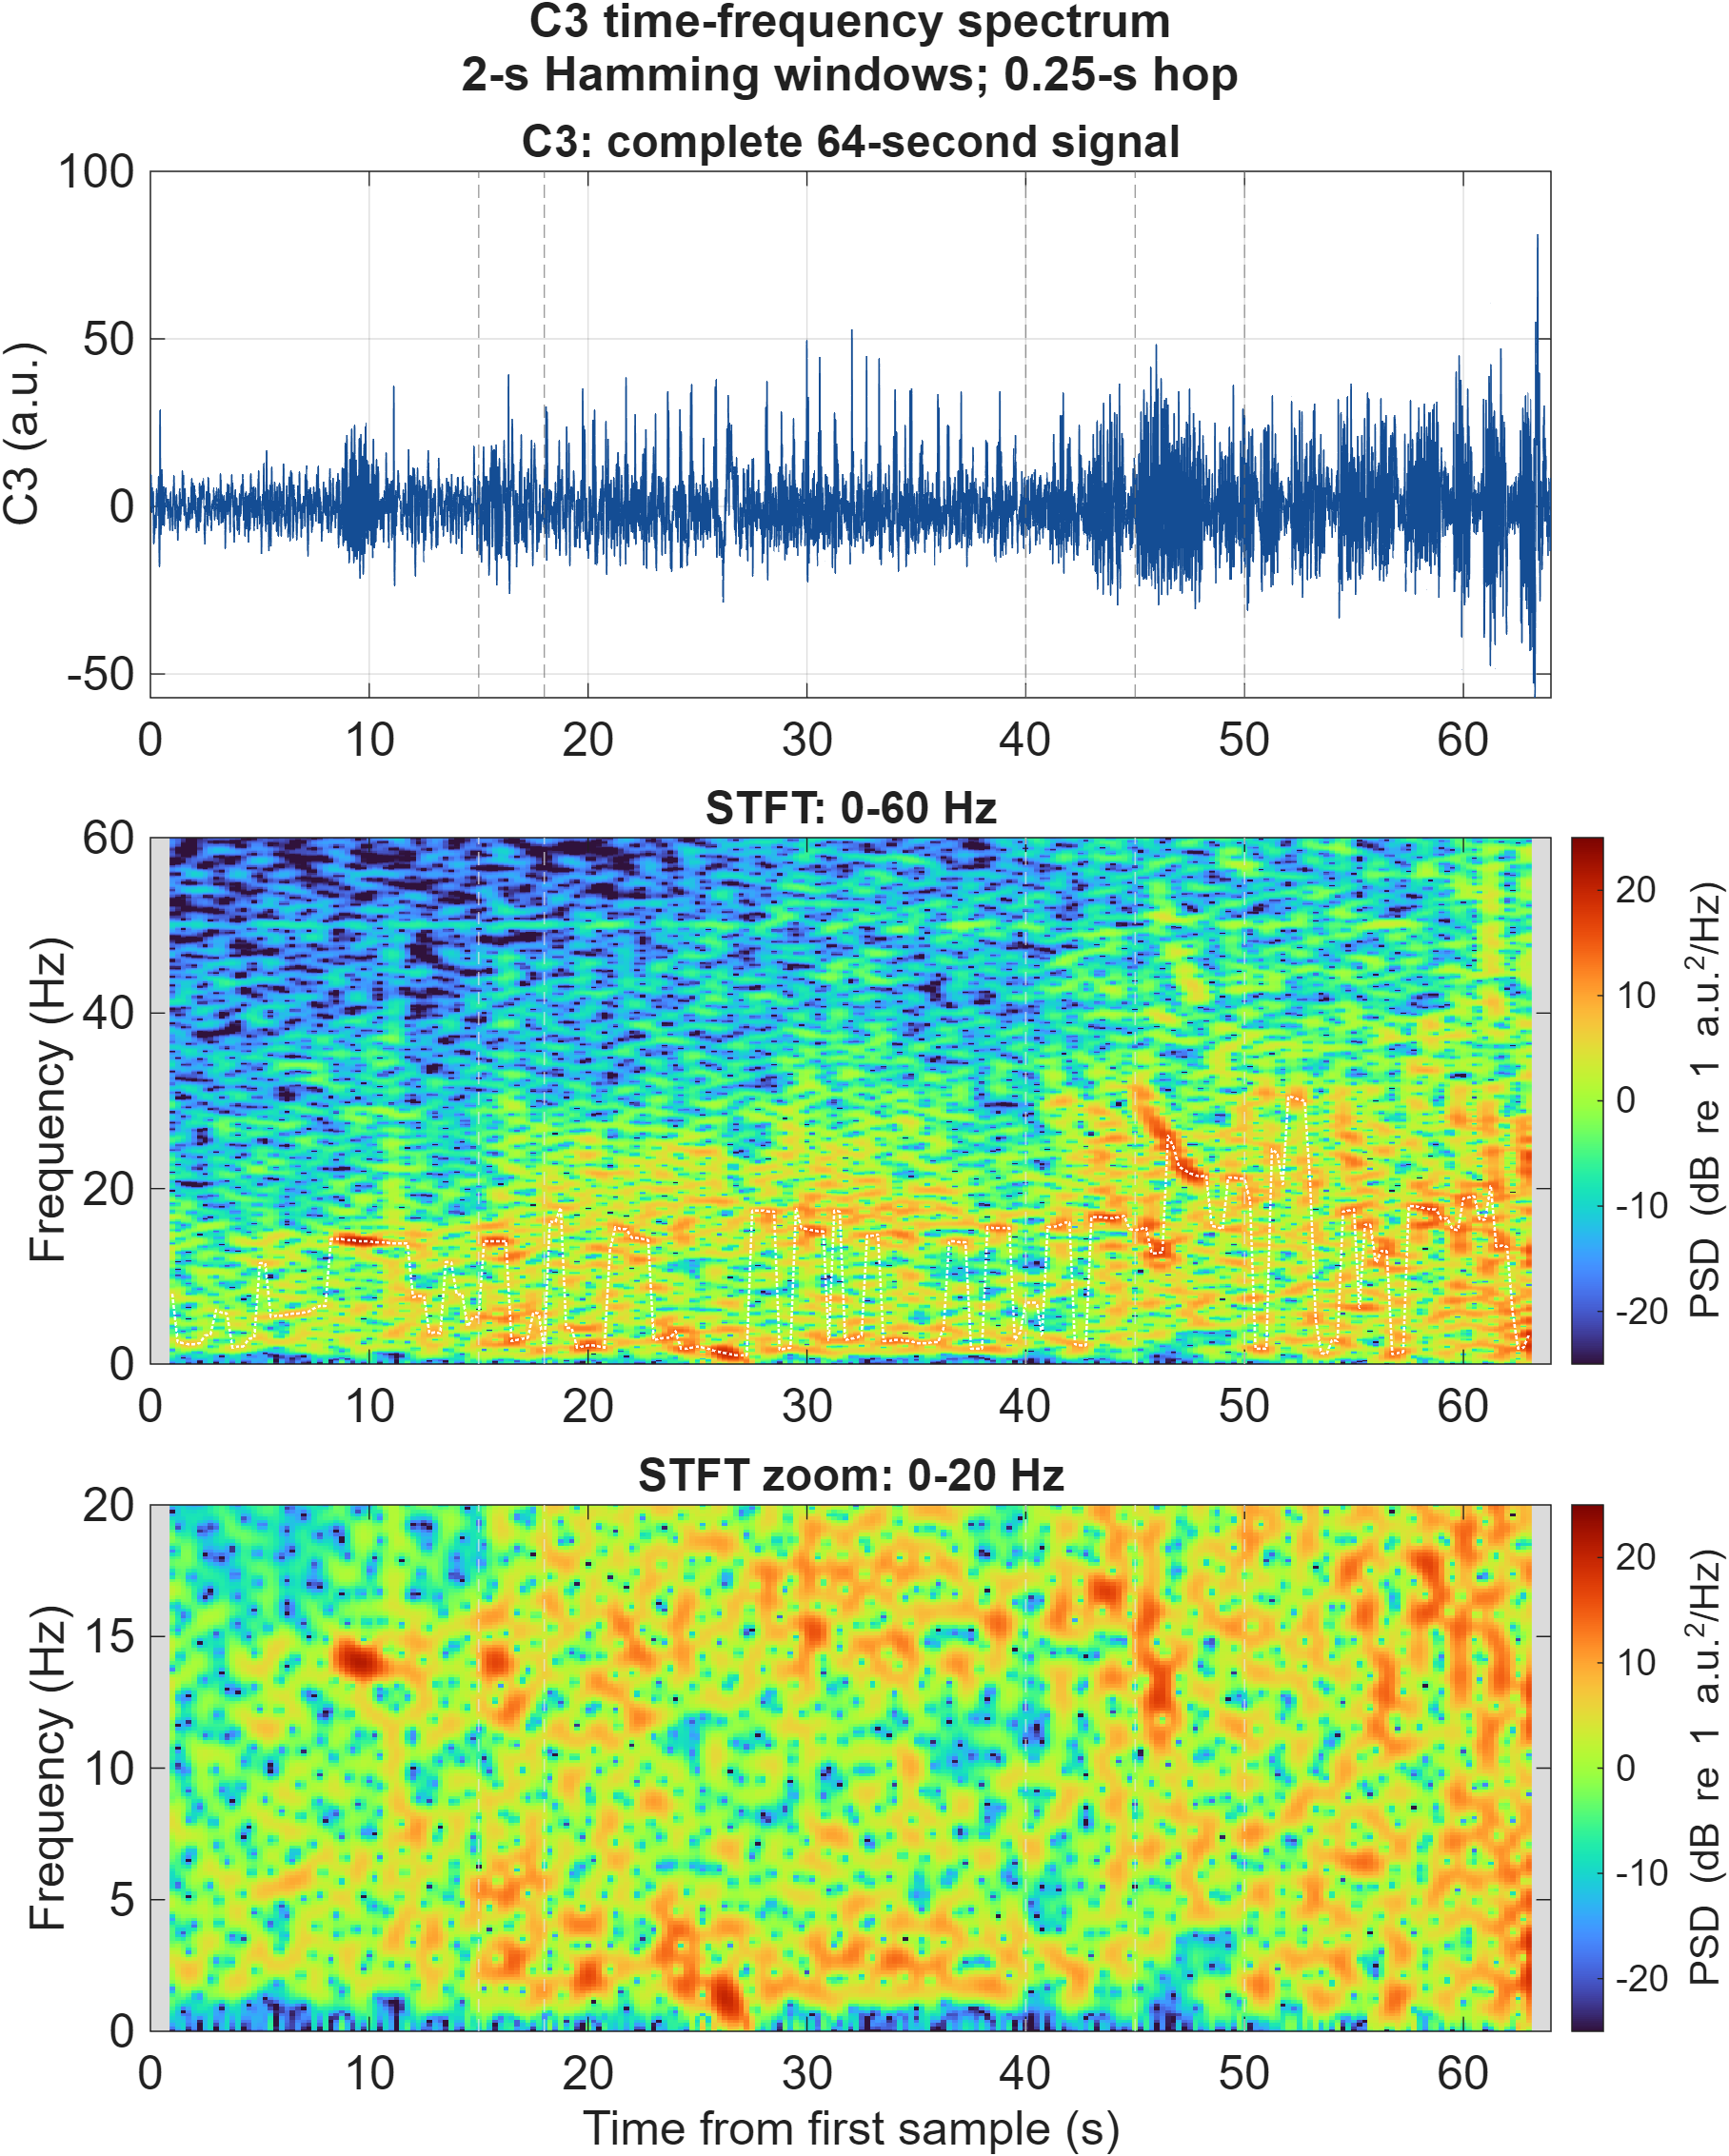
\includegraphics[width=0.82\textwidth]{fig02_c3_stft_full_recording.png}
\caption{Waveform and spectrogram of the whole C3 channel over 0--60~Hz and 0--20~Hz with the same color scale; the white line marks the strongest peak of each window, only within 1--40~Hz.}
\label{fig:c3stft}
\end{figure}

The times are window centers; the gray margins do not have a complete window. The spacing of the FFT grid is 0.125~Hz, but this value comes from zero-padding, and the true resolution is limited by the window length; the equivalent noise bandwidth of the window is about 0.68~Hz. This display complements Question~1 and does not change the settings requested for Question~8.

\subsection{Question 2: Examining Waveform Changes}
\begin{taskbox}
Examine the temporal-morphological features of the signal at different times (the first 15 seconds, approximately 18 to 40 seconds, approximately 45 to 50 seconds, and the final part from 50 seconds to the end of the signal). What notable features are seen in the signal?
\end{taskbox}

In the first 15 seconds, the background oscillations have a lower amplitude. In the range of 18 to 40 seconds, sharp discharges with a relatively regular repetition are seen on top of the background activity. In 45 to 50 seconds, the oscillations are denser and faster. From 50 seconds onward, the waves become more irregular and contain slower components and larger transients. In Figure~\ref{fig:c3four} each interval is displayed separately; the vertical scale of each panel must be read, and the apparent height on the page is not an independent measure of amplitude.

\begin{center}
\begin{tabular}{@{}ccc@{}}
\toprule
\textbf{Interval (s)} & \textbf{Peak-to-peak amplitude} & \textbf{AC RMS}\\
\midrule
0--15  & 59.41  & 6.09\\
18--40 & 81.34  & 8.79\\
45--50 & 78.80  & 12.50\\
50--64 & 138.08 & 13.18\\
\bottomrule
\end{tabular}
\end{center}

The amplitude values in the table are in a.u. The increase of the RMS from about 6.09 at the beginning of the recording to 13.18 at its end is consistent with the growth of amplitude. Nevertheless, part of the fast variation may be due to muscle artifacts, and its exact share cannot be separated from a single channel.

\begin{figure}[H]
\centering
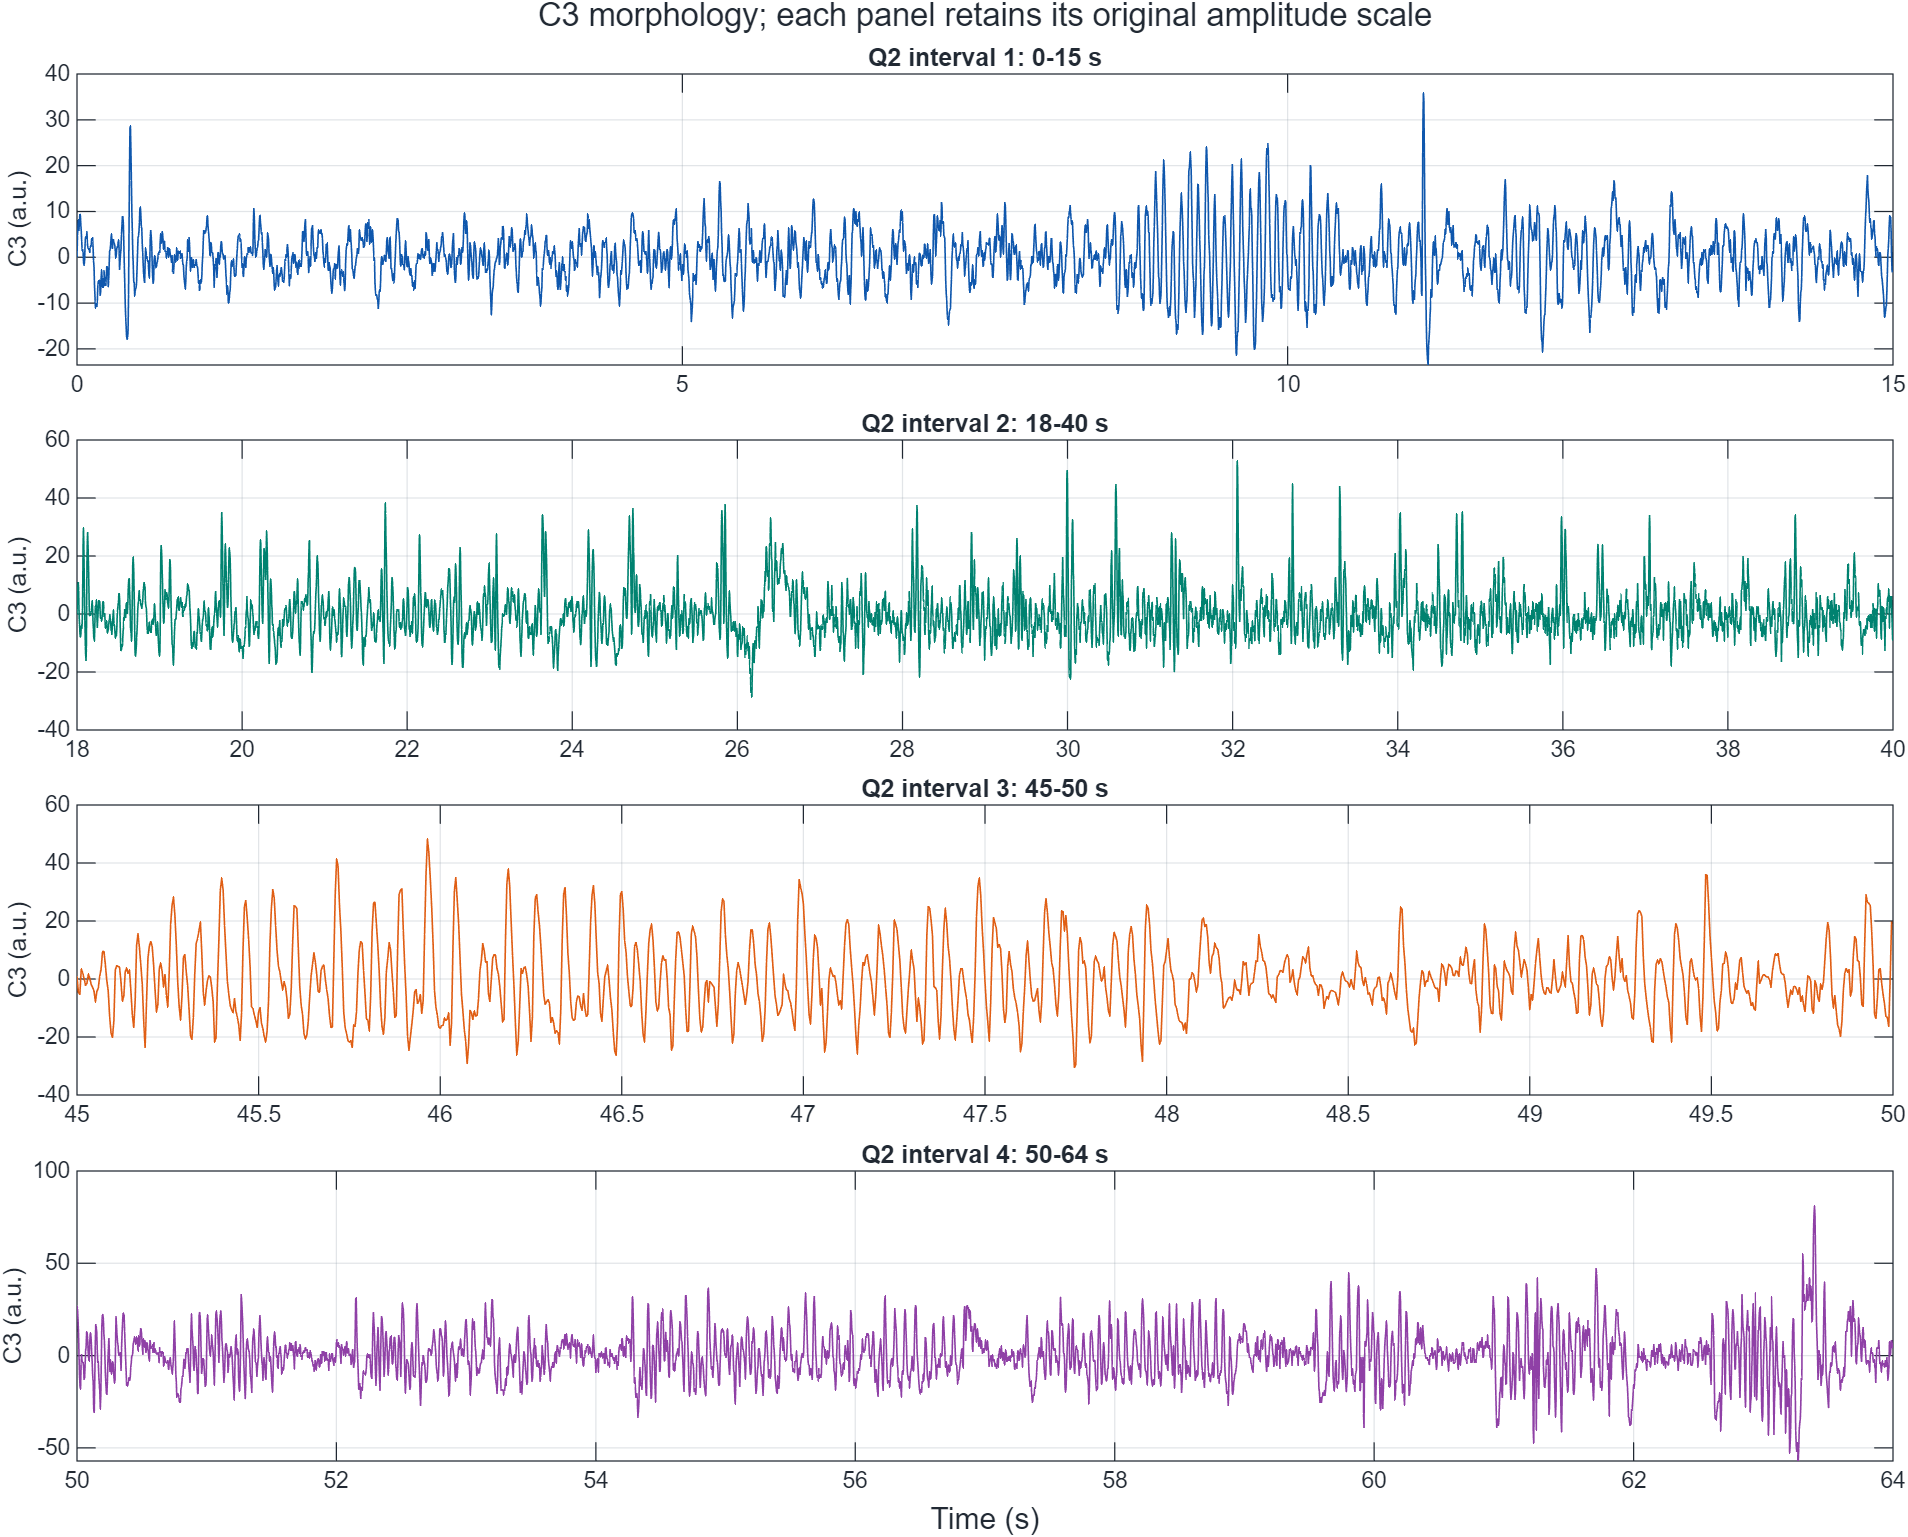
\includegraphics[width=\textwidth]{fig03_c3_four_intervals.png}
\caption{The four time intervals requested for examining the waveform shape of the brain channel.}
\label{fig:c3four}
\end{figure}

\subsection{Question 3: Comparison with Another Channel}
\begin{taskbox}
Plot another channel of your choice. Is the signal shape over time the same as in the 5th channel?
\end{taskbox}

Channel C4 was chosen for comparison with C3. The comparison of the two channels is shown in Figure~\ref{fig:c3c4}, and the display of all channels in Figure~\ref{fig:all32}.

\answer Overall, the signals of different channels share similarities in the general pattern of activity. For example, up to about second 27, and especially in the interval from 1 to 26 seconds, the general trend of variation is roughly similar. Nevertheless, the intensity, the time of occurrence and the clarity of the activities can differ from one channel to another, and some activities are not seen at the same level in all channels.

For instance, the relatively regular spikes present in channel C3 are seen in the other channels with the same regularity and prominence, or with a smaller amplitude. Also, the slower and more irregular envelopes seen in C3 from about second 40 onward do not appear in the same form in the other channels. By contrast, in the final part of the recording, high-power spikes are seen in different channels, which is one of the observable similarities among them.

\begin{figure}[H]
\centering
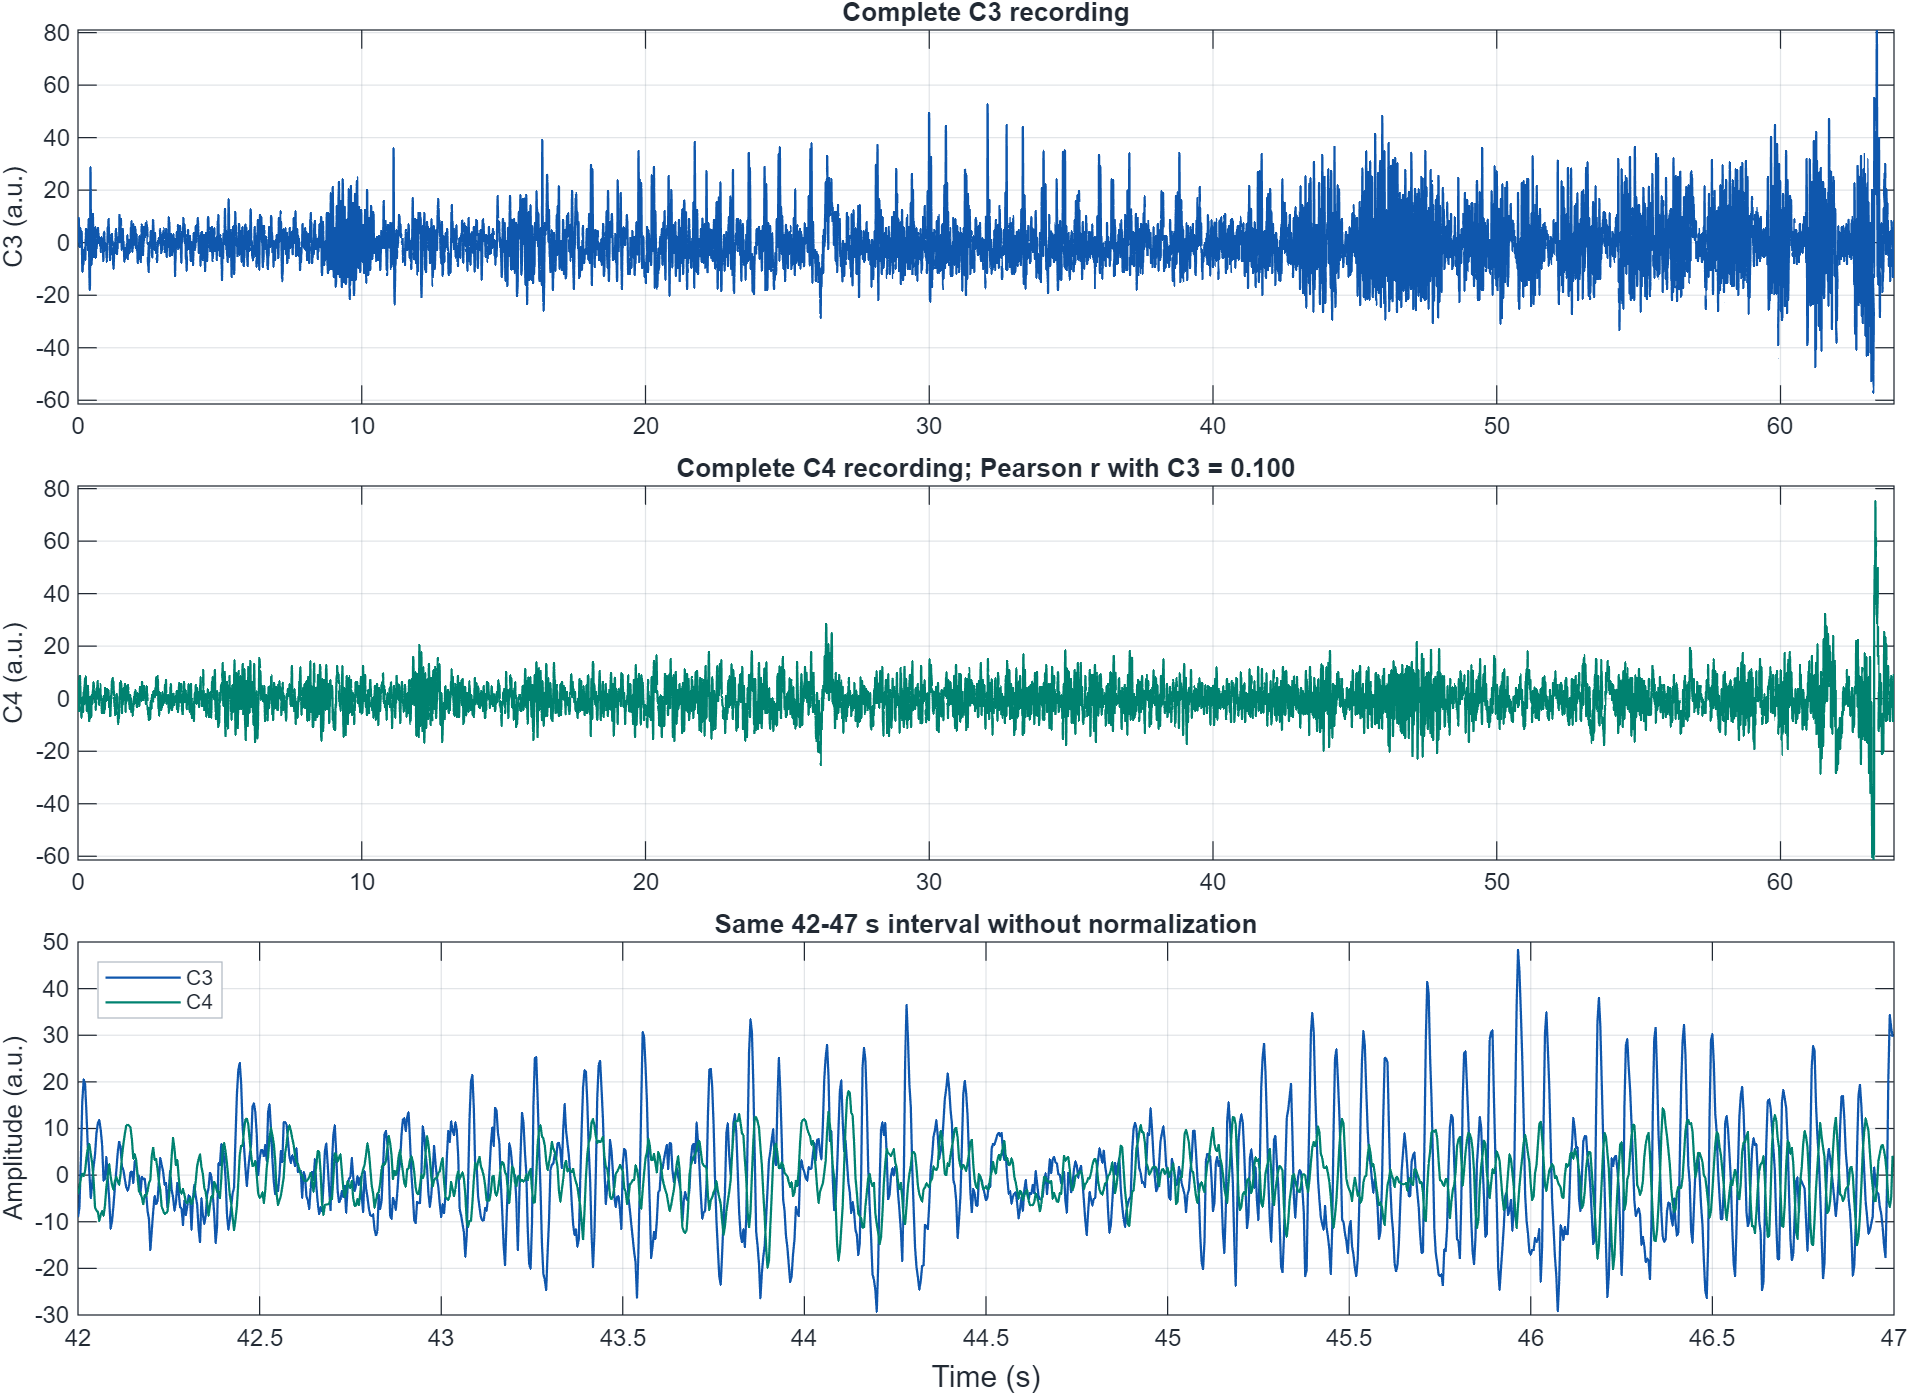
\includegraphics[width=\textwidth]{fig04_c3_c4_comparison.png}
\caption{Comparison of two central channels with common amplitude axes in the complete display.}
\label{fig:c3c4}
\end{figure}

\subsection{Question 4: Displaying All Channels}
\begin{taskbox}
Using the function \texttt{eeg\_disp} and the code snippet given in the manual, plot the EEG signal of all channels. For a better display, tune the variable \texttt{offset} (the spacing between the signals shown for two channels). Compare the behavior of the EEG signal in channel C3 (the 5th channel) with the other channels. C3 is close to the epileptic focus and clearly shows the changes of the EEG signal before and after seizure onset.
\end{taskbox}

All 32 channels were plotted with the original function \texttt{eeg\_disp}. The spacing between the channels follows the exercise: it equals the maximum absolute value of the data divided by five, about 87.50 units. This spacing is only a vertical offset for readability and is not added to the original data. The time vector of the accompanying function starts from $1/f_s$; in the output figure we aligned it with the common convention of starting from zero.

In Figure~\ref{fig:all32}, channel C3 is shown in blue. Its characteristics do not appear with the same intensity in all channels. For example, the correlation of CP1 with C3 is about 0.859 and that of FC1 about 0.741, whereas C4 has a lower correlation. This observation is consistent with the difference in recording location. The closeness of C3 to the focus is stated in the exercise; an independent localization of the focus from this plot was not performed.

\begin{figure}[p]
\centering
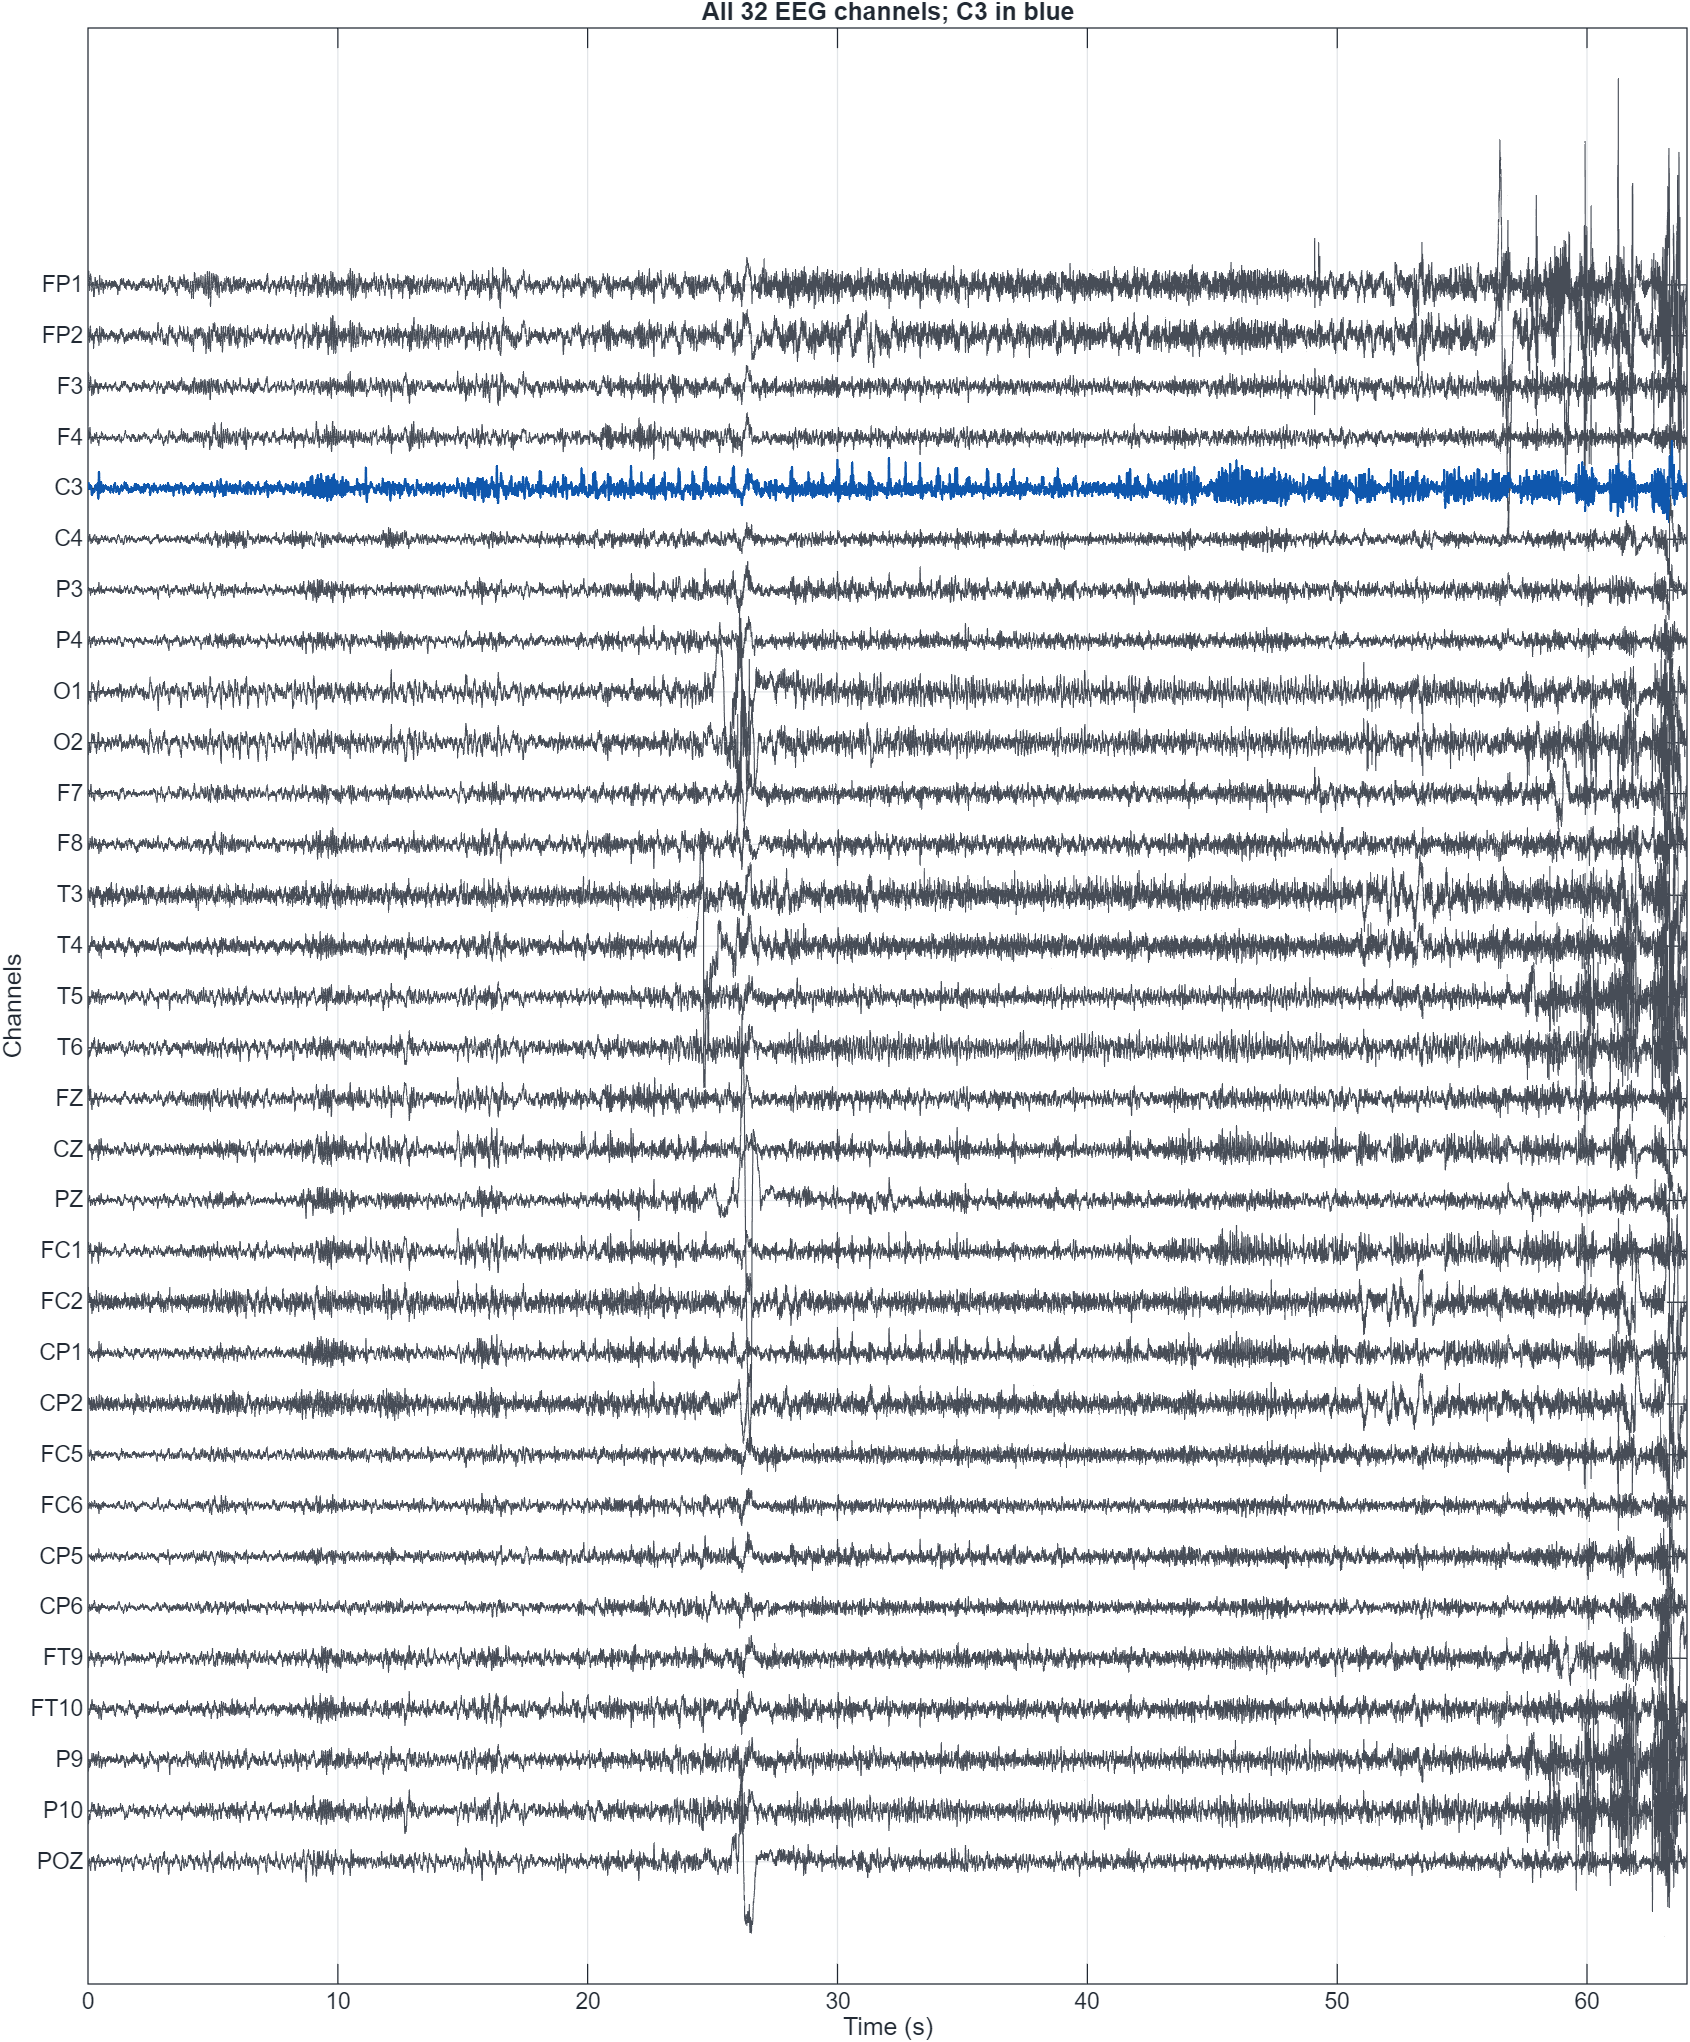
\includegraphics[height=0.78\textheight,keepaspectratio]{fig05_all_32_channels.png}
\caption{Display of all brain channels with a vertical offset, with the channel under study highlighted.}
\label{fig:all32}
\end{figure}

\subsection{Question 5: Interpreting the Three Sections of the Reference Figure}
\begin{taskbox}
Figure~1 of the manual shows the EEG signal of the first six channels. Research the characteristics of the signal in the three marked segments and summarize them briefly. (Caption of the manual's figure: a real EEG signal recorded from an epileptic patient during a seizure period, almost noise-free. Channel C3 shows seizure activity consisting of three parts: (1) rhythmic spikes before seizure onset (red box), (2) fast activity (green box) and (3) slower irregular activity (blue box).)
\end{taskbox}

\begin{figure}[H]
\centering
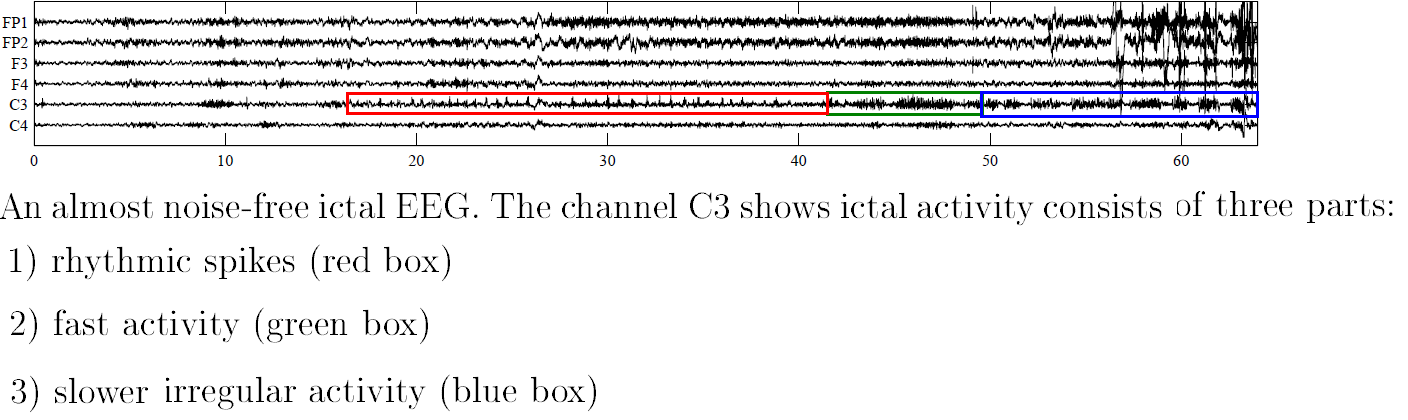
\includegraphics[width=\textwidth]{fig06_reference_ictal_figure.png}
\caption{The reference figure supplied with the data, for observing the three phases marked with colored frames. Its original caption reads: ``An almost noise-free ictal EEG. The channel C3 shows ictal activity consists of three parts: 1) rhythmic spikes (red box), 2) fast activity (green box), 3) slower irregular activity (blue box).''}
\label{fig:ref}
\end{figure}

Figure~\ref{fig:ref} is the reference image supplied with the experiment. The frame boundaries are approximate, and the three sections of channel C3 are interpreted on the basis of the waveform shape and its temporal evolution.

\paragraph{Red frame: rhythmic spikes before seizure onset.} At about 17 to 41.5 seconds, sharp, transient spikes repeat at relatively regular intervals. The title ``before seizure onset'' follows the Persian subtitle of the exercise statement; the exact electrographic onset of the seizure cannot be determined from the image alone. The repetition of the spikes creates periodicity, but their sharp shape also produces higher-frequency and harmonic components, so the repetition frequency is not the whole content of the spectrum. The presence of spikes alone is not sufficient for a definitive diagnosis or prediction of a seizure.

\paragraph{Green frame: fast activity.} At about 41.5 to 49.5 seconds, the oscillations become faster and more compact; their shorter temporal spacing is consistent with an increase in the higher-frequency content. The Welch peak at about 16.4~Hz and the larger beta share in the 42--47~s segment of the experiment data also support this description. Becoming faster is not necessarily an increase in amplitude; fast activity with low amplitude is also seen in some seizure-onset patterns.

\paragraph{Blue frame: slower and more irregular activity.} From about 49.5 seconds to the end, the activity is slower than in the green frame, and the spacing, shape and amplitude of the events are more variable. Slower components are prominent, but sharp transients can keep the spectrum broad. This part may be the evolution of the seizure activity itself; since the end of the attack is not marked and the exercise subtitle does not call it post-seizure, we do not take the slowing alone as equivalent to the end of the seizure.

The numerical values quoted here were computed from the data file, not from the image, and belong only to the corresponding segment. To compare intensity, the power or RMS must also be examined; a single spectral peak is not sufficient. The reference figure is described as almost noise-free, whereas the analyzed data contain artifacts; small differences between them are therefore not necessarily a contradiction.

\subsection{Question 6: Extracting Four Segments and the Fourier Transform}
\begin{taskbox}
Extract the following four 5-second segments from the C3 signal: 2 to 7~s, 30 to 35~s, 42 to 47~s and 50 to 55~s. Plot the time signal and the frequency spectrum (DFT) of each segment and give each figure a suitable title. Time and frequency must be displayed in seconds and Hz. Adjust the frequency axes so that the frequency content is displayed well (i.e., remove the high frequencies that carry no frequency information).
\end{taskbox}

Four segments, $(2,7]$, $(30,35]$, $(42,47]$ and $(50,55]$ seconds, were extracted. Each segment has exactly 1280 samples, and the spacing of the DFT points is 0.2~Hz. The mean was removed only for the spectral analysis. Figure~\ref{fig:dft4} shows the raw signal of each segment and its one-sided amplitude spectrum side by side. To see the main components, the frequency display is limited to 0--60~Hz; the full spectrum up to the Nyquist frequency is stored in the numeric file, and no display filter was applied.

\begin{figure}[H]
\centering
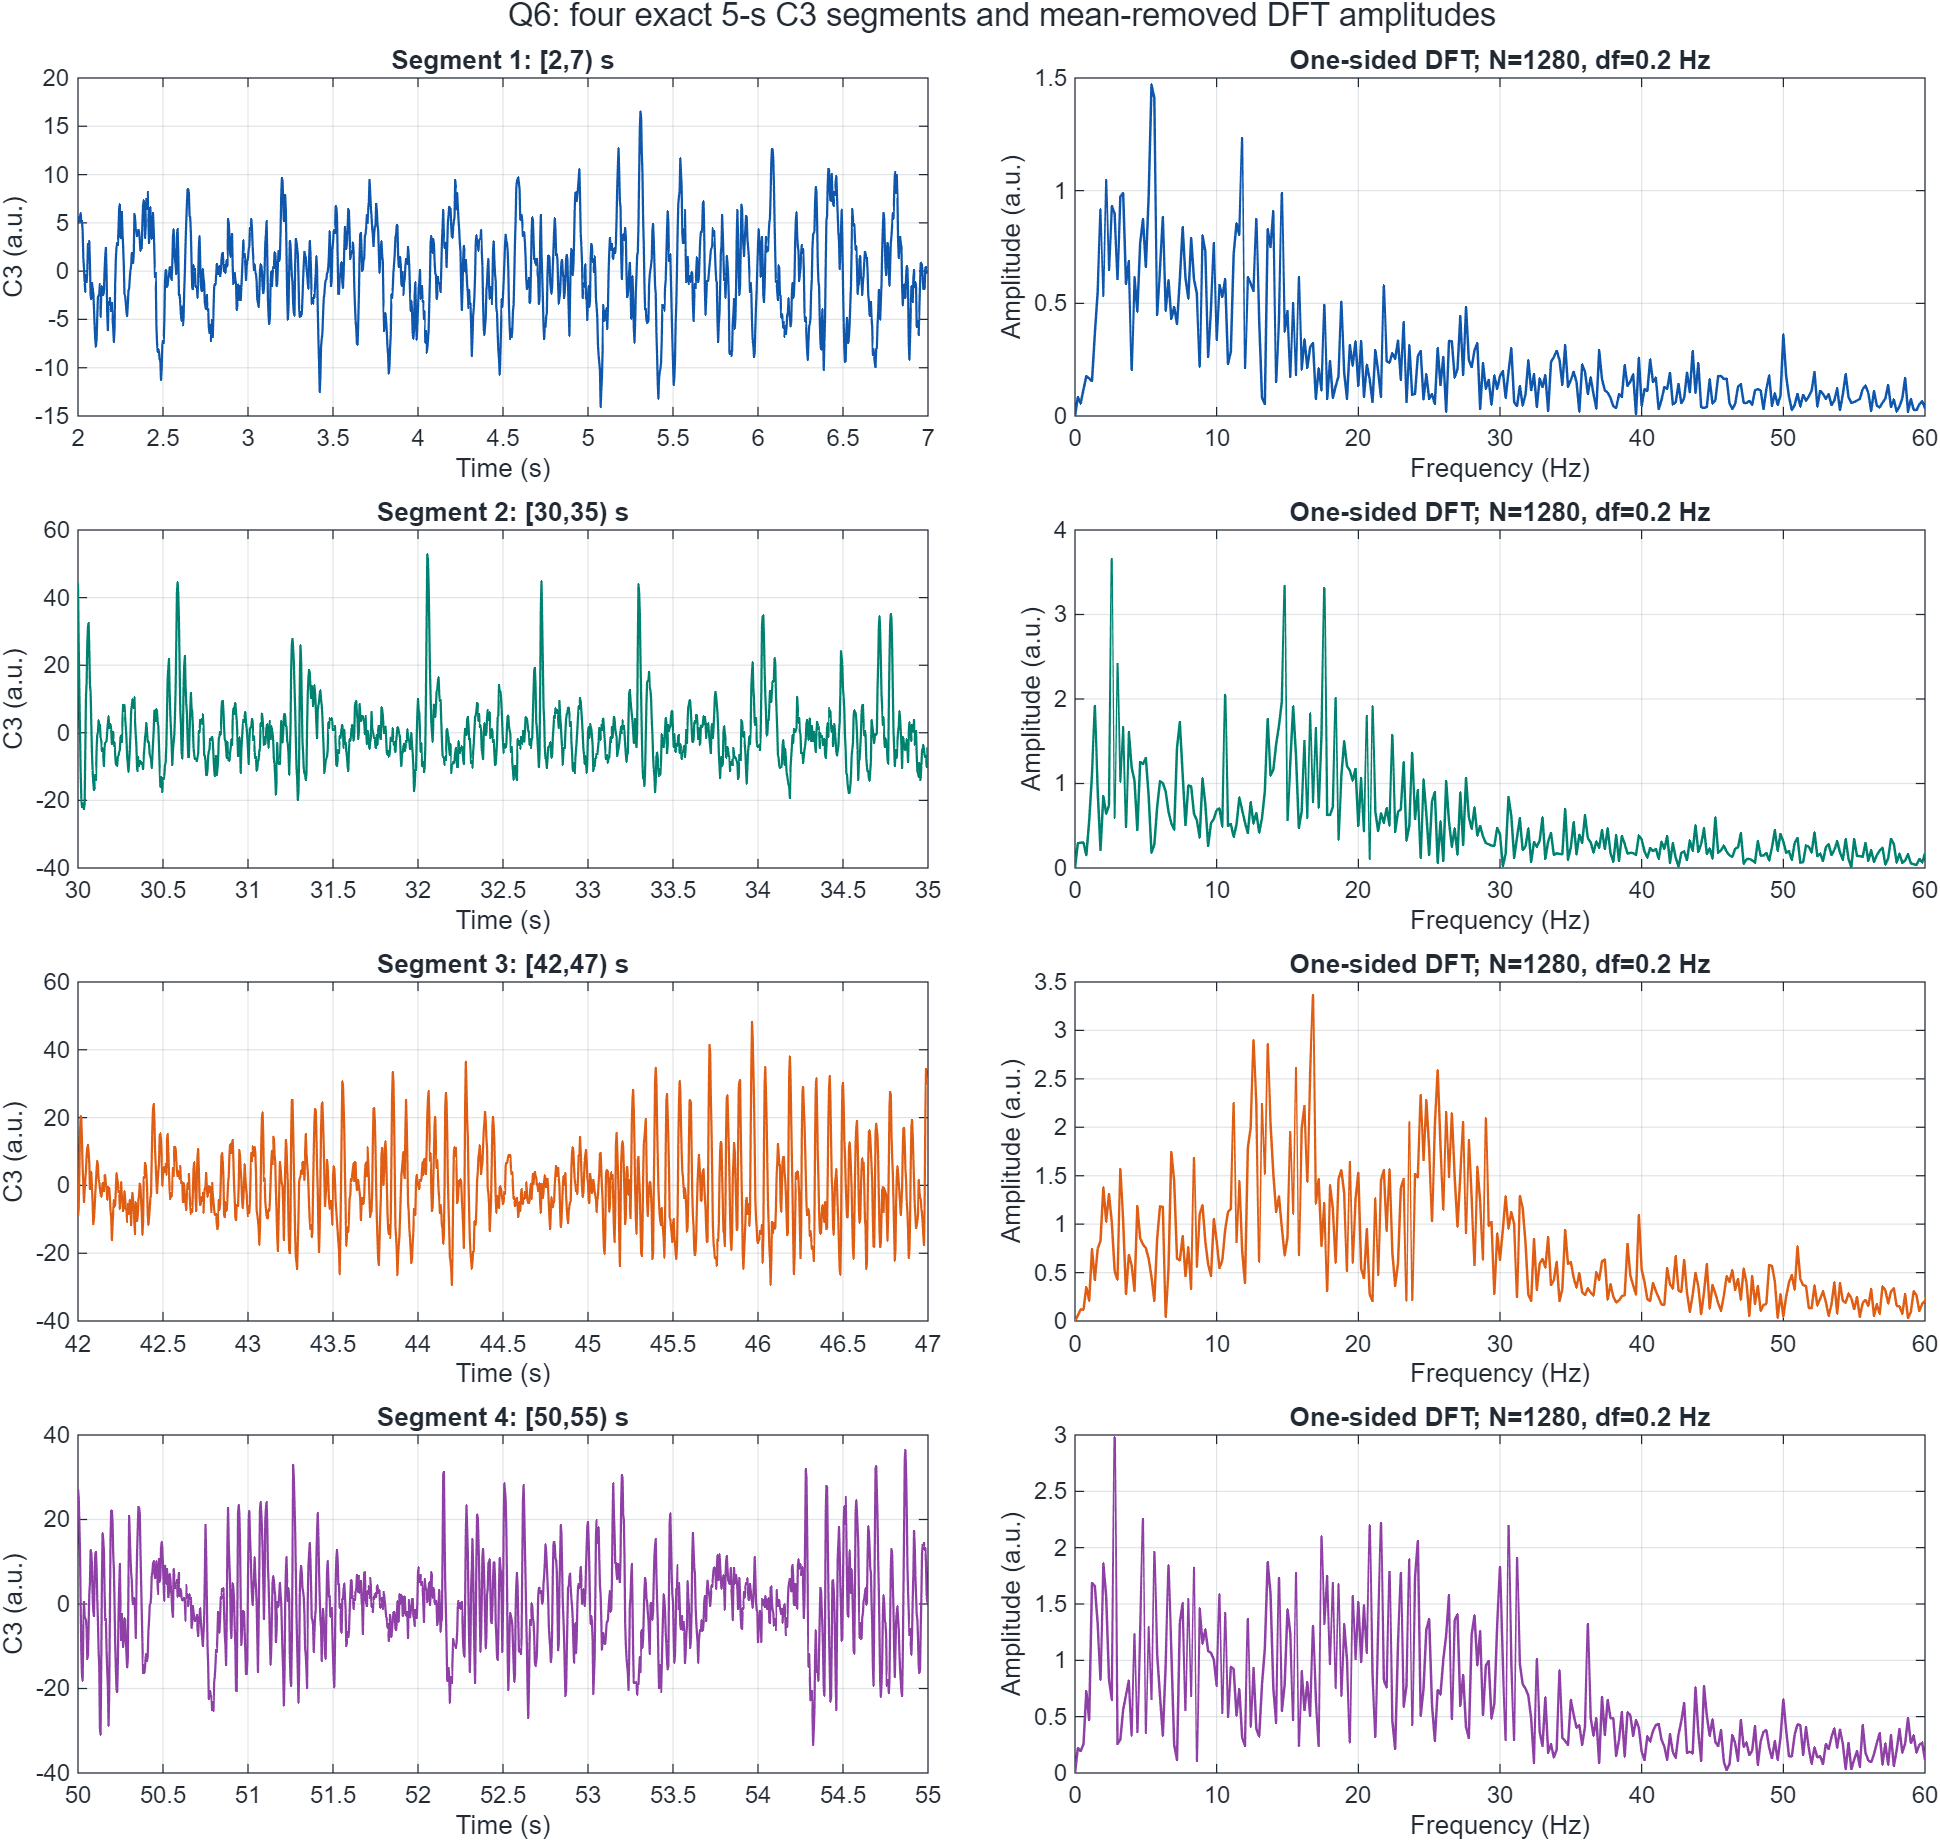
\includegraphics[width=\textwidth]{fig07_c3_segments_time_dft.png}
\caption{Time signal and amplitude spectrum of the four five-second segments with the correct DFT scaling.}
\label{fig:dft4}
\end{figure}

\subsection{Question 7: Spectrum Estimation with Welch's Method}
\begin{taskbox}
Plot the frequency spectrum of each of the four segments using the function \texttt{pwelch.m}. Set the input parameters so that the frequency content is displayed well. What can be said about the frequency characteristics of each of the four segments?
\end{taskbox}

For \texttt{pwelch}, a Hamming window of length 256, an overlap of 128 and \texttt{nfft=2048} at 256~Hz were used. Nine windows are averaged in each segment. The spacing of the plotting grid is 0.125~Hz; the intrinsic resolution of a one-second window remains of the order of 1~Hz. Besides the spectral peaks, Figure~\ref{fig:welch4} shows the increase in power of the second and third segments.

\begin{figure}[H]
\centering
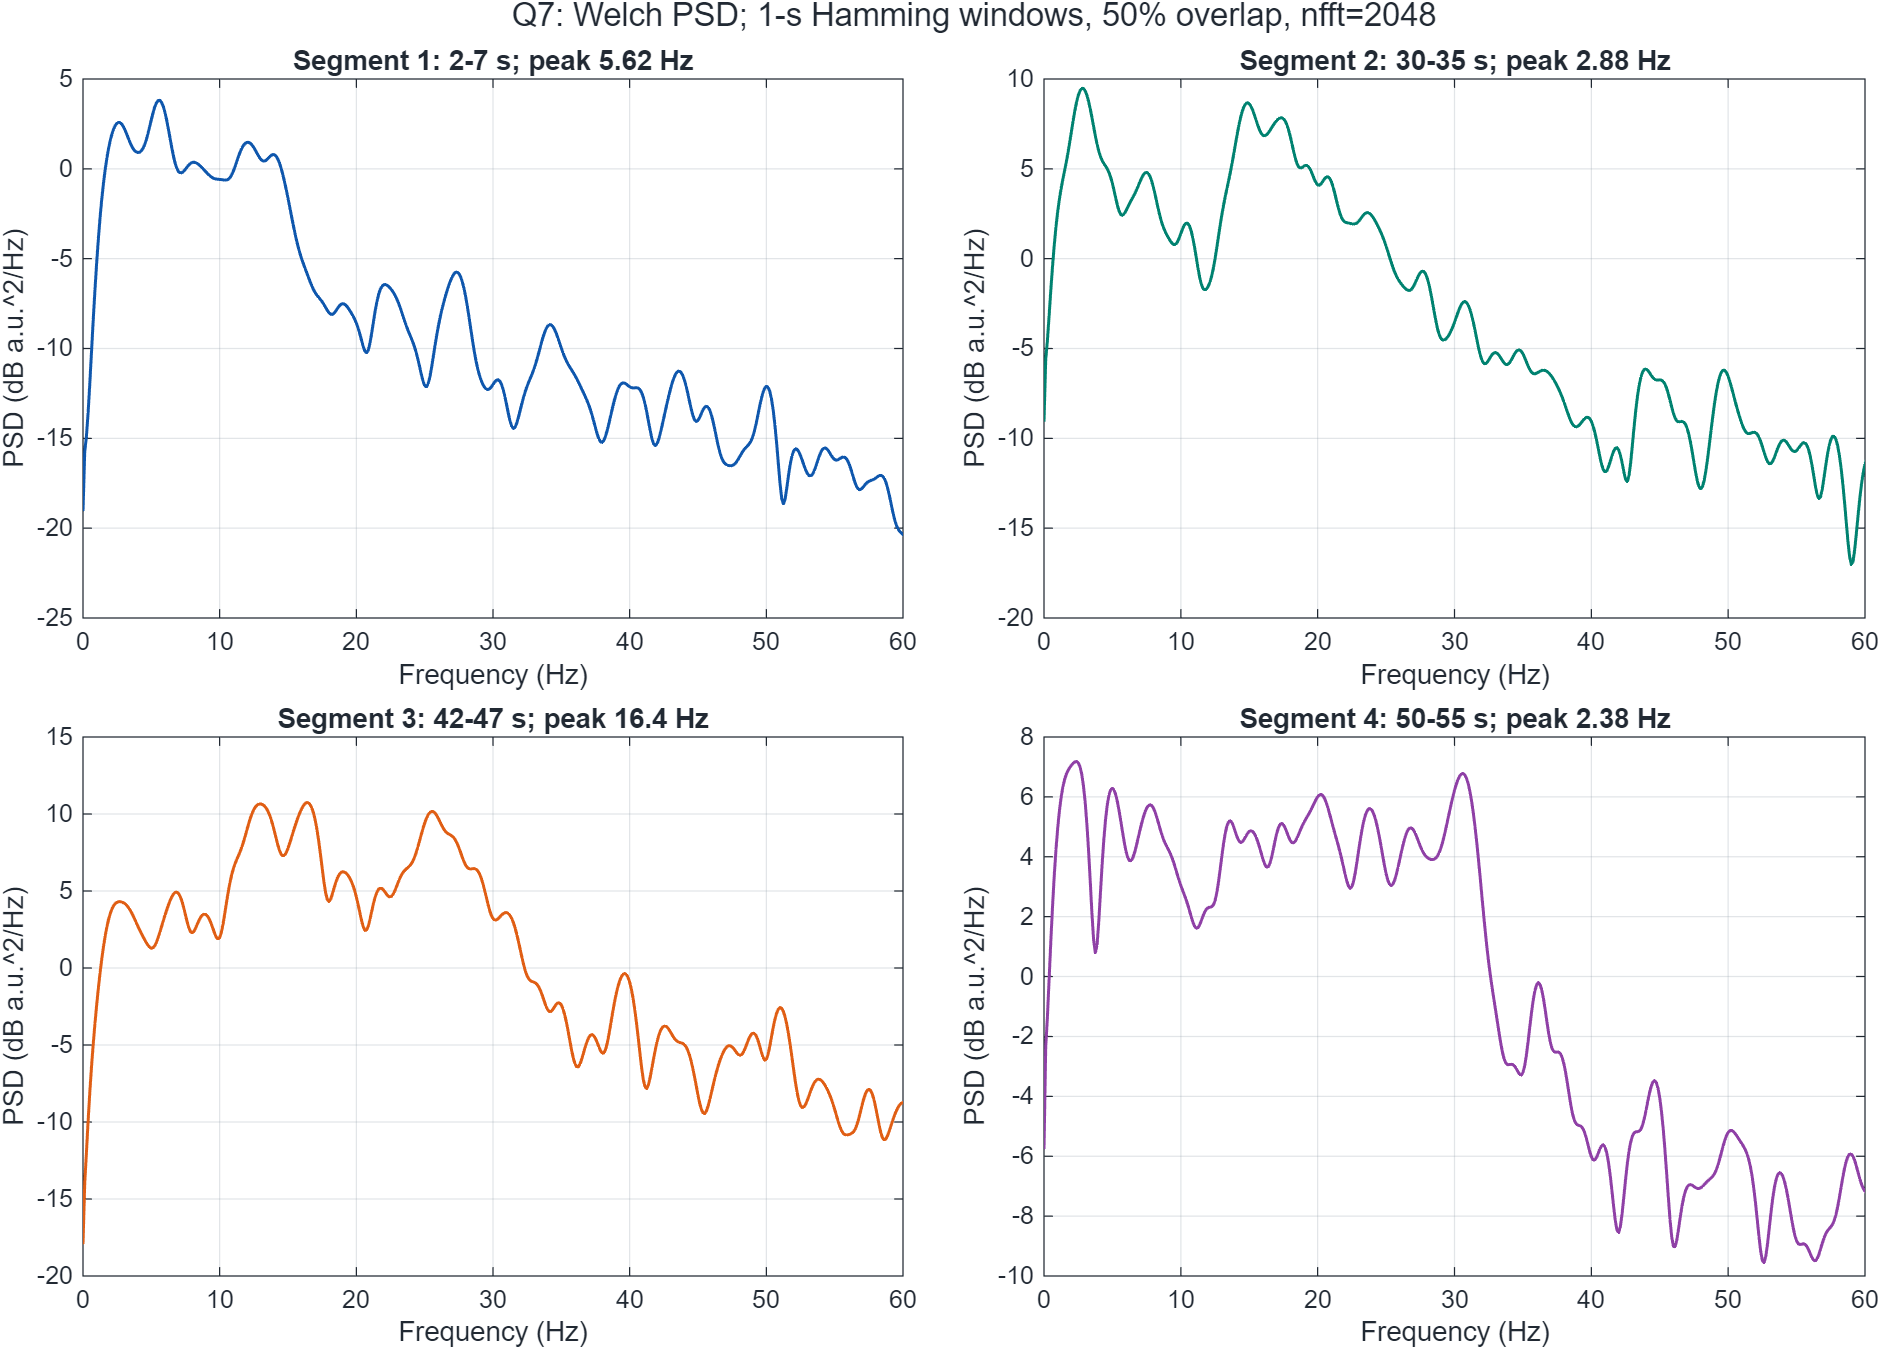
\includegraphics[width=0.95\textwidth]{fig08_welch_psd_segments.png}
\caption{Power spectral density of the four segments with fixed Welch settings.}
\label{fig:welch4}
\end{figure}

\begin{center}
\begin{tabular}{@{}ccccc@{}}
\toprule
\textbf{Interval (s)} & \textbf{AC RMS} & \textbf{Welch peak (Hz)} & \textbf{Beta share (\%)} & \textbf{Power above 60~Hz (\%)}\\
\midrule
2--7   &  4.58 &  5.625 & 21.97 & 1.44\\
30--35 &  9.61 &  2.875 & 52.92 & 2.09\\
42--47 & 12.14 & 16.375 & 64.82 & 1.72\\
50--55 & 10.81 &  2.375 & 47.32 & 2.71\\
\bottomrule
\end{tabular}
\end{center}

The beta share in the table was computed as the integral of power from 13 to 30~Hz divided by the power from 0.5 to 100~Hz. The share in the last column is relative to the total Welch power up to 128~Hz. These two denominators are different, and the values do not add up.

In the first segment, the main peak is at about 5.625~Hz, and the energy is distributed among the lower bands. In the second segment, the 2.875~Hz peak is consistent with the slow repetition of the spikes, but more than half of the power in the 0.5--100~Hz range lies in the beta band; the main peak alone therefore does not describe the width of the spectrum. The third segment has a peak at 16.375~Hz and a beta share of about 64.82\%, and it shows the fast activity more clearly. The peak of the fourth segment returns to 2.375~Hz, but the fast content and the artifacts have not completely disappeared.

\subsection{Question 8: Spectrogram with the Specified Settings}
\begin{taskbox}
Using the \texttt{spectrogram} command with window length $L=128$, an overlap of $N_{\mathrm{overlap}}=64$ points and $n_{\mathrm{fft}}=L=128$, compute and plot the time--frequency spectrum of the four segments using a Hamming window (time and frequency axes in seconds and Hz, respectively). What can be said about the time--frequency characteristics of each of the four segments?
\end{taskbox}

The parameters were set exactly to $L=128$, $N_{\mathrm{overlap}}=64$, $n_{\mathrm{fft}}=128$ and a Hamming window. As a result, the window length is 0.5~s, the time step is 0.25~s and the frequency spacing is 2~Hz. Each segment has 19 time frames. The color in Figure~\ref{fig:stft4} is in decibels of power spectral density, with common limits in all panels.

\begin{figure}[H]
\centering
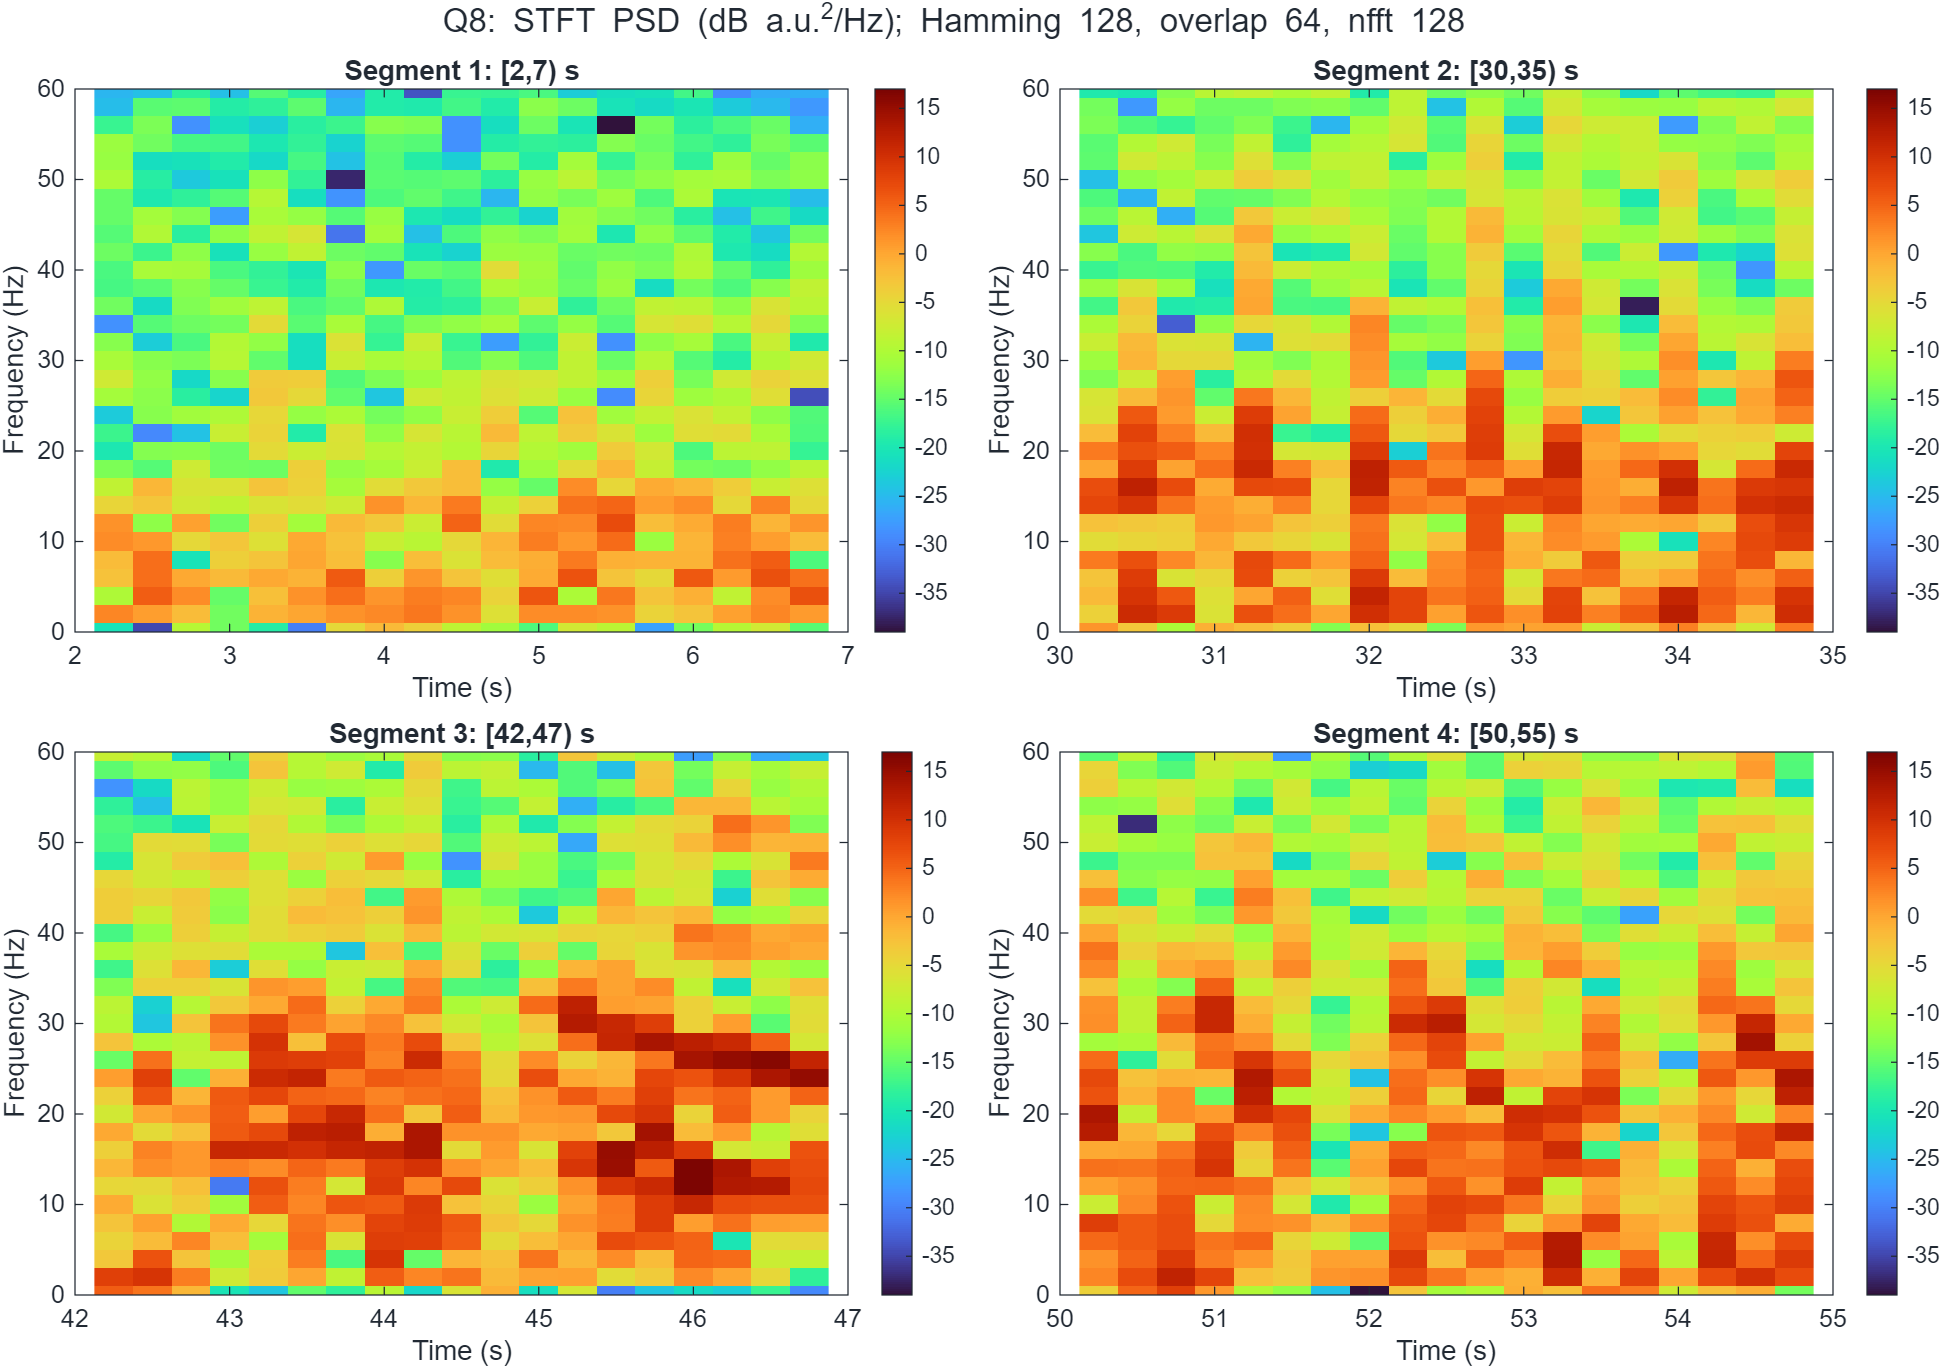
\includegraphics[width=0.95\textwidth]{fig09_stft_segments.png}
\caption{Spectrogram of the four segments with the exactly requested window and overlap.}
\label{fig:stft4}
\end{figure}

\answer In the first segment, the power is lower and the activity has a smaller amplitude. The second segment shows repeating temporal variations and the simultaneous presence of slow and fast components; the wide-band transient stripes are consistent with the sharpness of the spikes. In the third segment, the energy in the beta range and around 16~Hz is more prominent. In the fourth segment, the distribution of power is more irregular, and slow components are accompanied by fast transients. This display shows that two segments with similar overall spectra can have different temporal ordering; a stationary spectrum alone does not reveal this difference.

\subsection{Question 9: Reducing the Sampling Rate and Checking Information Preservation}
\begin{taskbox}
Consider the signal of segment 2. Since the sampling frequency is relatively high, assume that the obtained frequency spectrum is similar to the spectrum of the continuous signal. Under this assumption, and using the information obtained in Questions 6 and 7, reduce the sampling frequency (downsampling) such that the frequency content is preserved. Before reducing the sampling rate, use a suitable low-pass filter. Plot the time signal, the frequency spectrum (DFT) and the STFT of the new signal, and compare them with the results of the previous parts.
\end{taskbox}

For the second segment, downsampling by a factor of two, from 256 to 128~Hz, was chosen. In the raw recording, the power above the new Nyquist frequency is not zero: about 1.85\% of the Welch power lies above 64~Hz, and the bandwidth containing 99\% of the power is about 84.5~Hz. Complete preservation of the full bandwidth of the recording at 128~Hz is therefore not possible. The purpose of this choice is an approximate preservation of the main brain band and a controlled reduction of the fast content of the recording.

A low-pass filter with a passband edge of 48~Hz, a stopband start of 64~Hz, a single-pass ripple of 0.1~dB and a single-pass attenuation of 60~dB was designed. \texttt{filtfilt} was run on the whole channel, then every other sample was kept, and finally the same time interval was extracted. In this way, the two edges of the segment use the actual neighboring samples for filtering, and the forward--backward phase delay is removed. The effective amplitude response is the square of the single-pass response; a maximum passband deviation of about 0.170~dB and a stopband attenuation of about 120~dB were measured.

\begin{center}
\begin{tabular}{@{}lr@{}}
\toprule
\textbf{Index} & \textbf{Value}\\
\midrule
Number of samples before / after the reduction & 1280 / 640\\
Duration of both segments (s) & 5\\
Share of the main power below 48~Hz & 96.56\%\\
Ratio of the filtered time-domain power to the raw & 97.14\%\\
Correlation with the corresponding raw samples & 0.9862\\
Relative difference of the Welch spectrum in 0.5--40~Hz & 0.327\%\\
Relative difference of the spectrogram below 40~Hz & 1.462\%\\
\bottomrule
\end{tabular}
\end{center}

The correlation of about 0.986 and the difference of about 0.327\% in the Welch spectrum in the 0.5--40~Hz band show that the main part of the oscillations was preserved. The difference from the raw data is intentionally non-zero; the RMSE of the retained samples is about 1.609~a.u. We therefore do not claim a lossless reconstruction for the whole recording. Figure~\ref{fig:ds} presents the comparison of time, amplitude, power density and the filter response.

\begin{figure}[H]
\centering
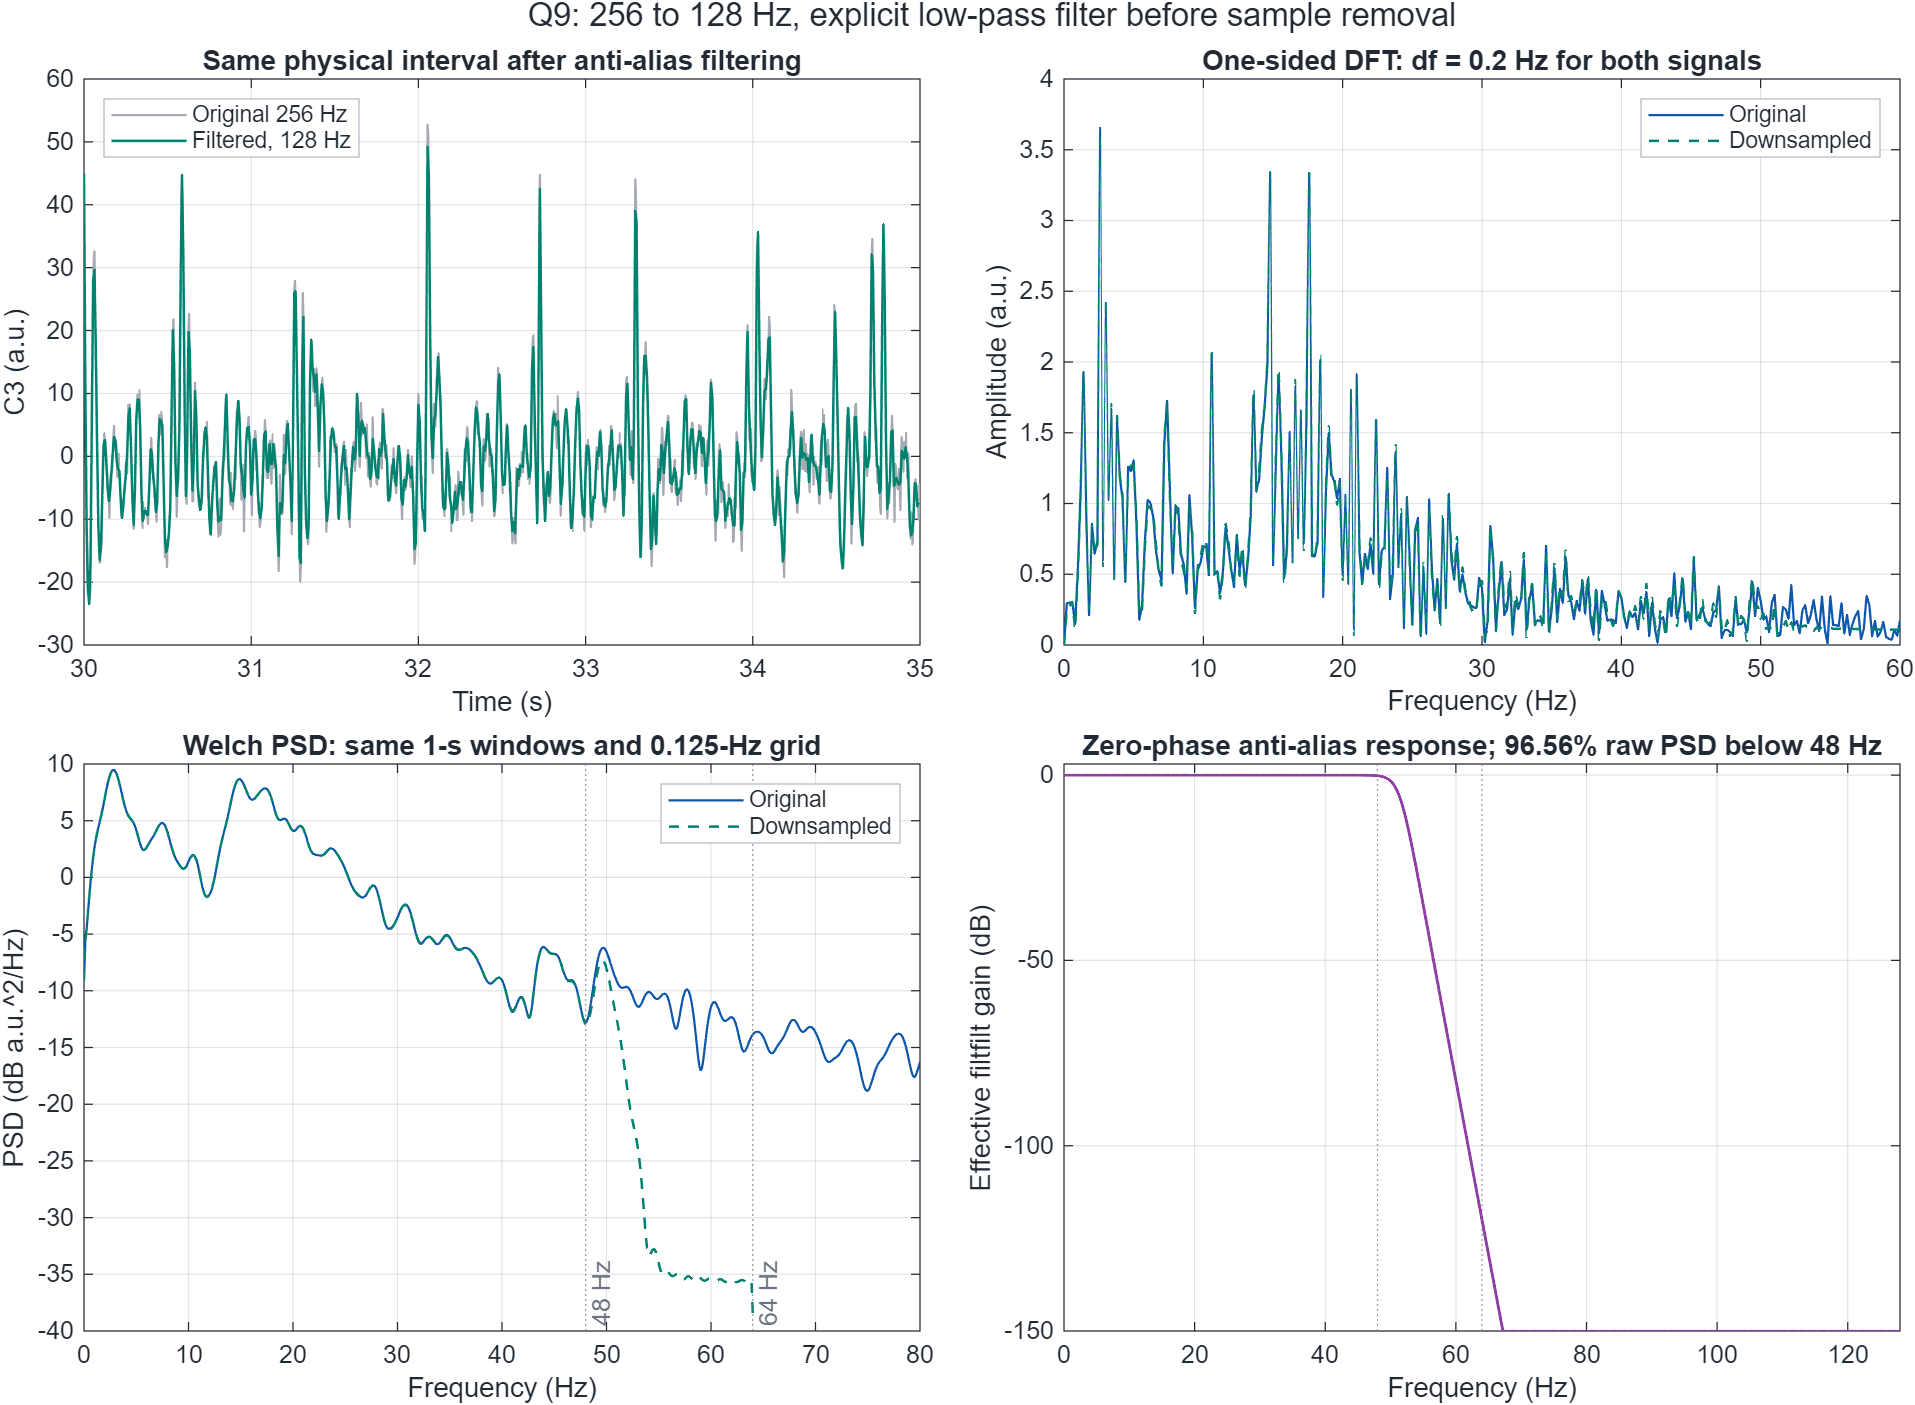
\includegraphics[width=\textwidth]{fig10_downsampling_comparison.png}
\caption{Comparison before and after reducing the sampling rate, and examination of the anti-aliasing filter response.}
\label{fig:ds}
\end{figure}

For a fair comparison of time and frequency, the physical length of the window was kept fixed. At the new rate, the spectrogram window has 64 samples, an overlap of 32 and \texttt{nfft=64}; the window is therefore still half a second long and the frequency spacing is still 2~Hz. Reusing the length of 128 samples at the new rate would have made the window one second long and mixed the effect of the rate reduction with the effect of changing the window. Figure~\ref{fig:dsstft} shows the similarity of the original time--frequency pattern on compatible grids.

\begin{figure}[H]
\centering
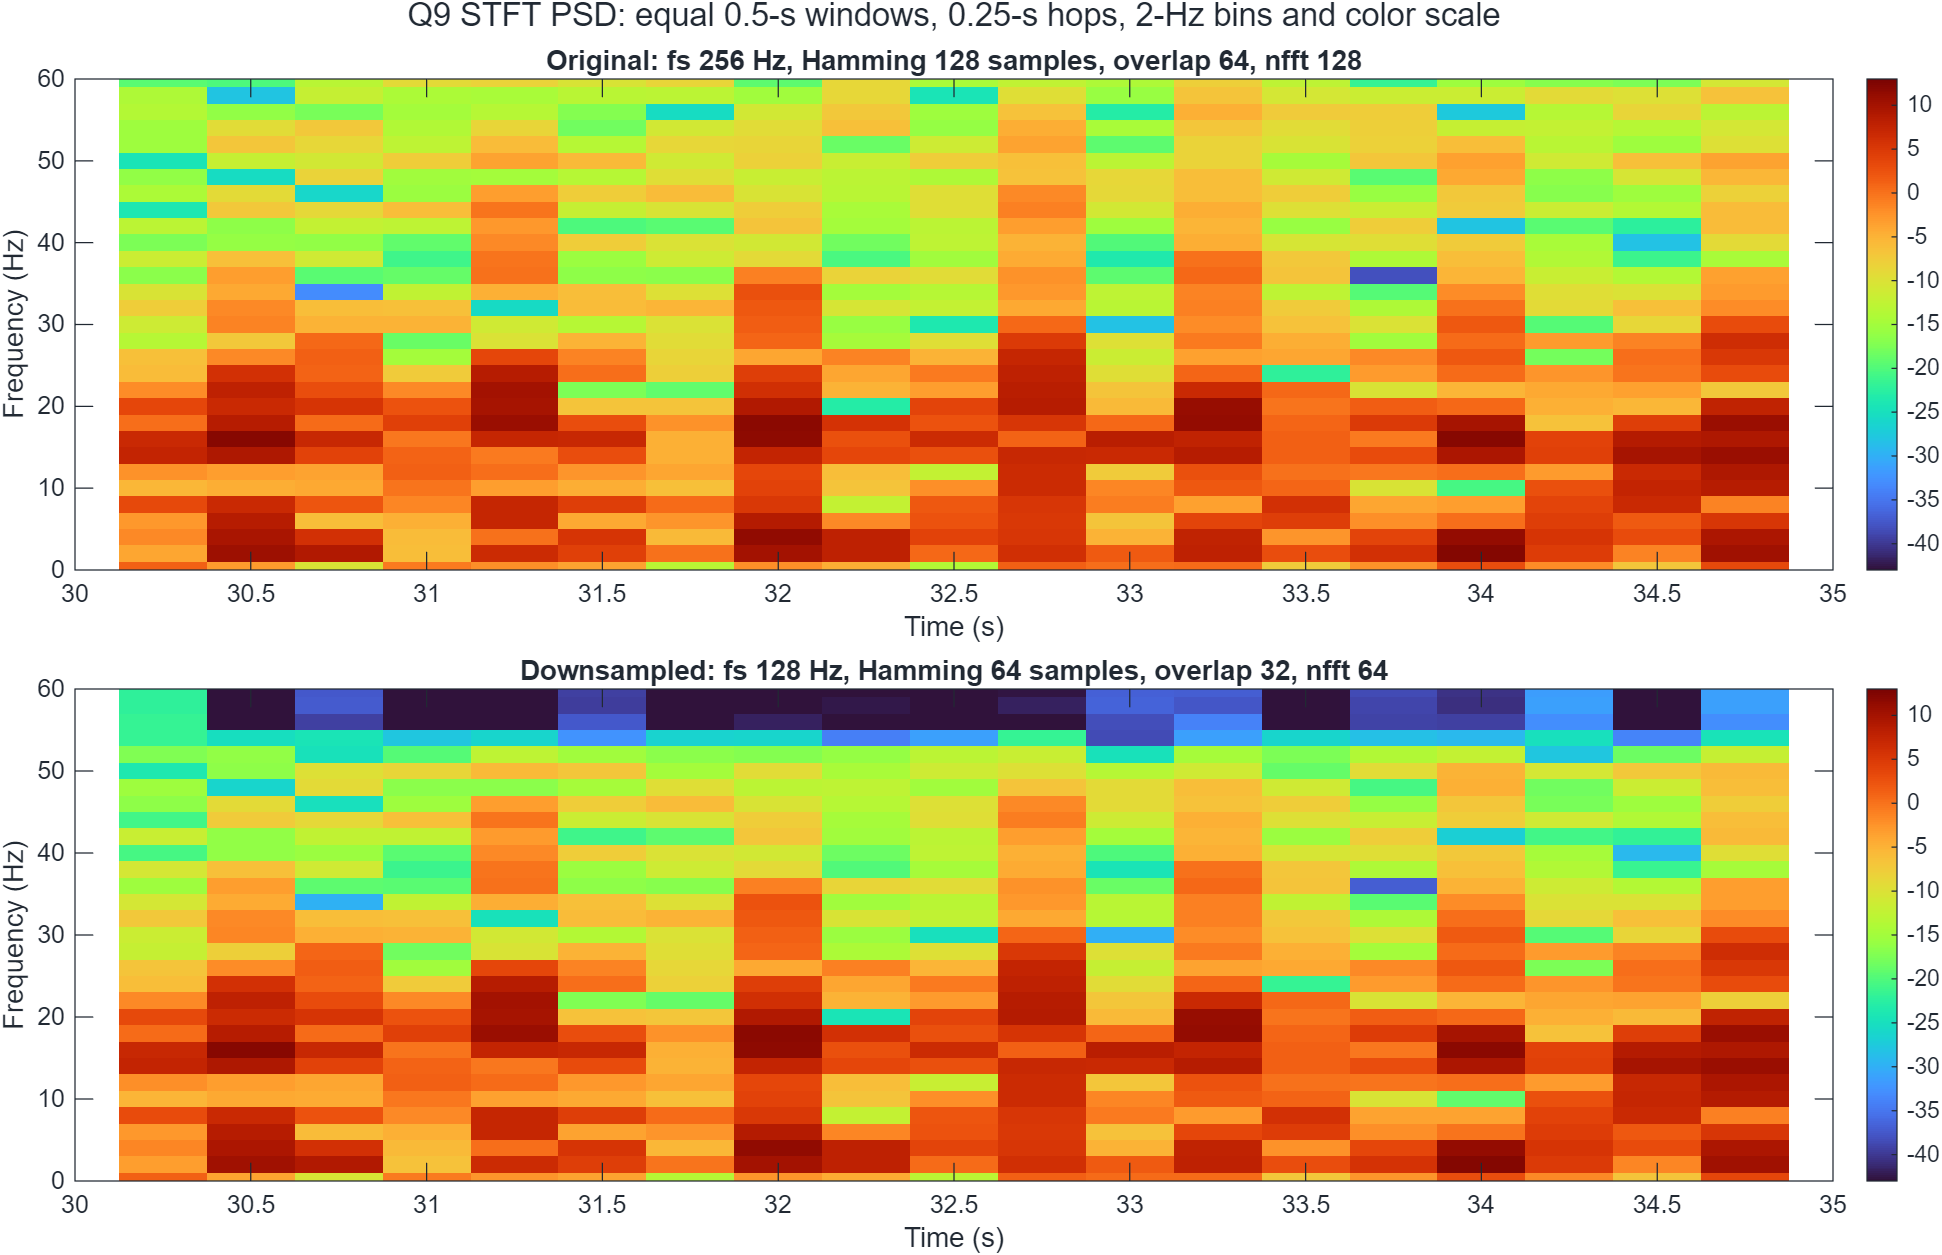
\includegraphics[width=0.95\textwidth]{fig11_stft_before_after_downsampling.png}
\caption{Comparison of the spectrogram before and after the reduction, with the same window duration and a common color scale.}
\label{fig:dsstft}
\end{figure}

\subsection{Core Implementation (EEG)}

\begin{lstlisting}[language=Matlab]
fs = des.samplingfreq;
t = (0:size(Z,2)-1)/fs;
idx = round(30*fs)+1 : round(35*fs);
x = Z(5,idx);                      % Exactly 1280 samples
[P,f] = pwelch(x-mean(x),hamming(256),128,2048,fs);
[S,F,T,Ptf] = spectrogram(x-mean(x),hamming(128),64,128,fs);
\end{lstlisting}

The motivation for this code is to avoid a one-sample error in slicing and to build the frequency axis from the actual recording rate. The complete code for filtering, extracting the indices and saving the figures is in \texttt{code/lab1\_eeg.m}.
